\section{Related Work}
\label{sec:relatedwork} 

\subsection{What does ``quality'' mean?}

Despite multiple publications about requirements quality and its assessment, 
the term ``quality'' is still subjective~\cite{Mund:2017},~\cite{Femmer:2017}. 
Industry standards~\cite{ISO/IEC/IEEE:2011} specify characteristics and criteria, 
which presumed effective for improving requirements quality, e.g, completeness, unambiguity. 
Additionally, the research community provided several types of quality definition and methods for its assessment. 
For example, Lamsweerde provides a defect-based checklist to inspect requirements for possible flaws 
and errors in ~\cite{Lamsweerde:2009}; Pohl proposes a framework defining dimensions of quality: 
the specification dimension, the representation dimension, the agreement dimension~\cite{POHL:1994}.
This approach considers such imprecise and subjective attributes as requirements adequacy or pertinence, thereby purporting uncertain assessment.
Instead of analyzing the meaning of the requirements, our method takes into account a maturity of the whole requirements artifact (RA).

%This approach purports an uncertain assessment due to impreciseness of the considered attributes, 
%such as requirements adequacy or pertinence. Instead of such level of granularity for requirements 
%consideration, our method take into account a requirements artifact (RA) in general. 

Another approach implies syntactic check of the requirements text for improving its comprehension, 
correctness, ambiguity and other akin characteristics e.g.~\cite{Ferrari:2014},~\cite{Berry:2006}.
All these metrics apply intrinsic inspection of requirements and assess qualitatively the requirements' statement. 
In contrary, our metrics provide a \textit{quantitative} analysis of a full document with the requirements.

In comparison with methods described above, activity-based quality models shift their approach from inherent properties of the requirements 
to the context of process, and propose a meta quality model~\cite{Wagner:2012},~\cite{Femmer:2015}. 
Furthermore, the "quality question" also turns to a consideration of how the requirements quality impacts the project success and the relation between 
them in scientific community~\cite{Emam:1995},~\cite{Kamata:2007}, so as among practitioners~\cite{BeattyHokanson:2014}.

\begin{figure}[H]
	\centering
		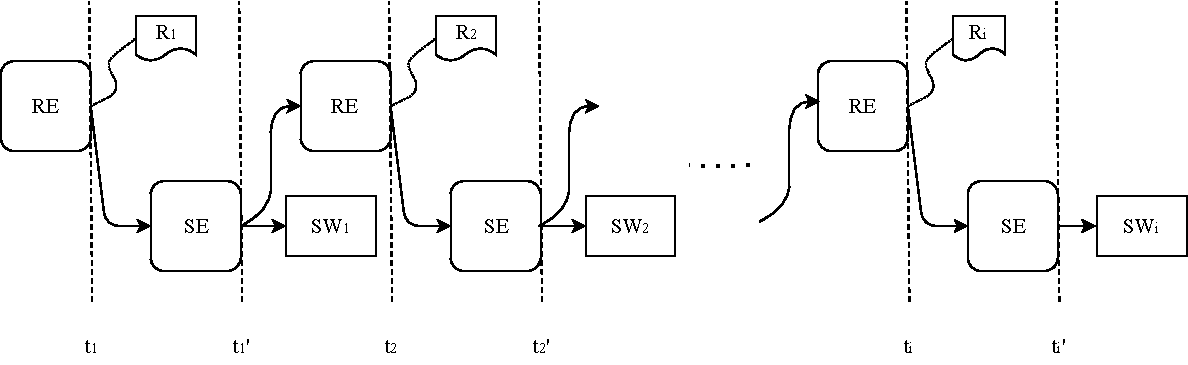
\includegraphics[width=1.00\textwidth,height=2in]{MetricsDiag.pdf}
	\caption{Requirements engineering and development processes}
	\label{fig:Metrics_shot}
\end{figure}

In contrast to the approaches, our metrics grant a quick and lightweight method for the quality assessment considering the number of the requirements' corrections.
%our metrics grant a relative simplicity level and provide a precision with cardinal number in assessment.

%Pleiad 
A series of studies about the relation between quality and project outcomes, ~\cite{Verner:2005},~\cite{Kamata:2007},~\cite{Noorwali:2015} triggers our research to the proposed metrics. Scientific papers investigating maturity of requirements~\cite{Basili:1981},~\cite{FARBEY:1990} and their complexity~\cite{Antinyan:2016} give a base for the idea of transforming a relation between requirements quality and number of changes in requirements document into quantitative measurement, but they described the quality aspects within the ongoing process. The metrics presented in this paper consider a requirements artifact as a ``black box'' for its maturity and a process of adjusting the requirements at RE and implementation phases, in a quantitative way, once a project is over.

%Now exists a vast majority of quality definitions:
%\begin{enumerate}
	%\item in industry Standards - set of attributes such as completeness, unambiguity... [ISO/IEC/IEEE-29148];
	%\item in scientific point of view, [Lamsweerde] gives a general list of characteristics, [Pohl] proposed a framework defining dimensions of quality (• the specification dimension, • the representation dimension, the agreement dimension.);
	%\item check requirements language for lacking of errors, defects, ambiguity and possible reasons for incomprehension [];
	%\item different kind of quality models such as activity-based[10], natural-language requirements specifications[7] %(activity, stupid!)
%\end{enumerate}
%
%
%\subsection{Metrics for quality measure}
%\begin{itemize}
	%\item methodology for context-specific RE artifact quality measuring has in its base an activity-based quality model [activity, stupid!] - brief description
	%\item the mentioned attributes should be satisfied 
	%\item some researchers shift their look to product quality measurement e.g [measuring success], however 
%\end{itemize}
%
%All these metrics intend to intrinsic inspection of requirements. In contrast to them, we propose the quantitative metrics for assessment of requirements quality